\begin{minted}[autogobble]{python}
import numpy as np
import matplotlib.pyplot as plt
from mpl_toolkits.mplot3d import Axes3D

Lx = 2
Ly = 1
H = 0.001  # 1mm
nx = 21
ny = 10
alpha = 111e-6  # 111mm^/s

x_vals = np.linspace(0, Lx, nx)
y_vals = np.linspace(0, Ly, ny)
points = np.array(np.meshgrid(x_vals, y_vals, indexing="ij")).T.reshape(-1, 2)
n = points.shape[0]
i0 = np.where((points[:, 0] != Lx) & (points[:, 1] != Ly))[0]  # 0-index
elements = np.array([[i0,i0],[i0 + 1, i0 + nx + 1],[i0 + nx + 1, i0 + nx]]).T.reshape(-1, 3)
m = elements.shape[0]
element_h = np.repeat(H,m)
element_centers = (points[elements[:, 0],:] + points[elements[:, 1],:]+points[elements[:, 2],:]) / 3

sel = (element_centers[:,0] > Lx * 0.3) & (element_centers[:,0] < Lx * 0.7) & (element_centers[:,1] > Ly * 0.5)
element_h[sel] = H / 10

plt.tripcolor(points[:,0],points[:,1],elements,facecolors=element_h)
plt.show()
\end{minted}

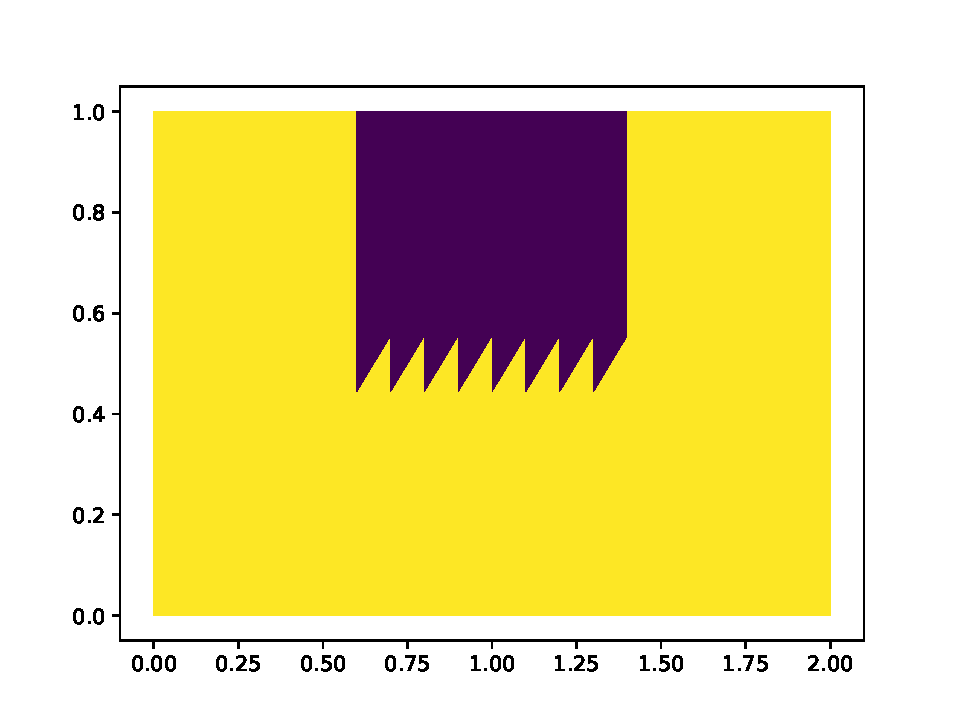
\includegraphics{heat_files/figure-latex/unnamed-chunk-1-1.pdf}

\begin{minted}[autogobble]{python}
dofs = n
RHS = np.zeros(dofs)
S = np.zeros((dofs, dofs))
M = np.zeros((dofs, dofs))

for el, h in zip(elements, element_h):
    J = np.array([points[el[1],:]-points[el[0],:],points[el[2],:]-points[el[0],:]])
    local_dof = el
    tmp1 = np.linalg.det(J) * np.linalg.inv(np.dot(J.T, J))
    tmp2 = np.array([[-1, 1, 0], [-1, 0, 1]])
    local_S = np.dot(np.dot(tmp2.T, tmp1), tmp2) * h * alpha
    S[np.ix_(local_dof, local_dof)] += local_S
    local_M = np.linalg.det(J) * np.array([[2, 1, 1], [1, 2, 1], [1, 1, 2]]) / 24
    M[np.ix_(local_dof, local_dof)] += local_M

plt.imshow(S)
plt.show()
\end{minted}

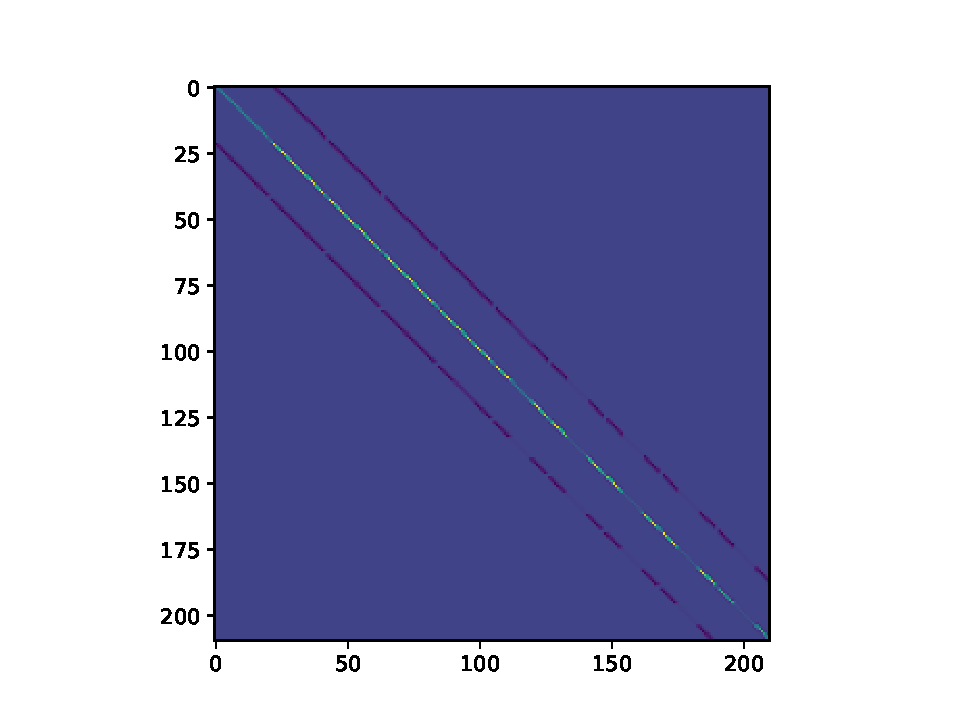
\includegraphics{heat_files/figure-latex/unnamed-chunk-1-2.pdf}

\begin{minted}[autogobble]{python}
plt.imshow(M)
plt.show()
\end{minted}

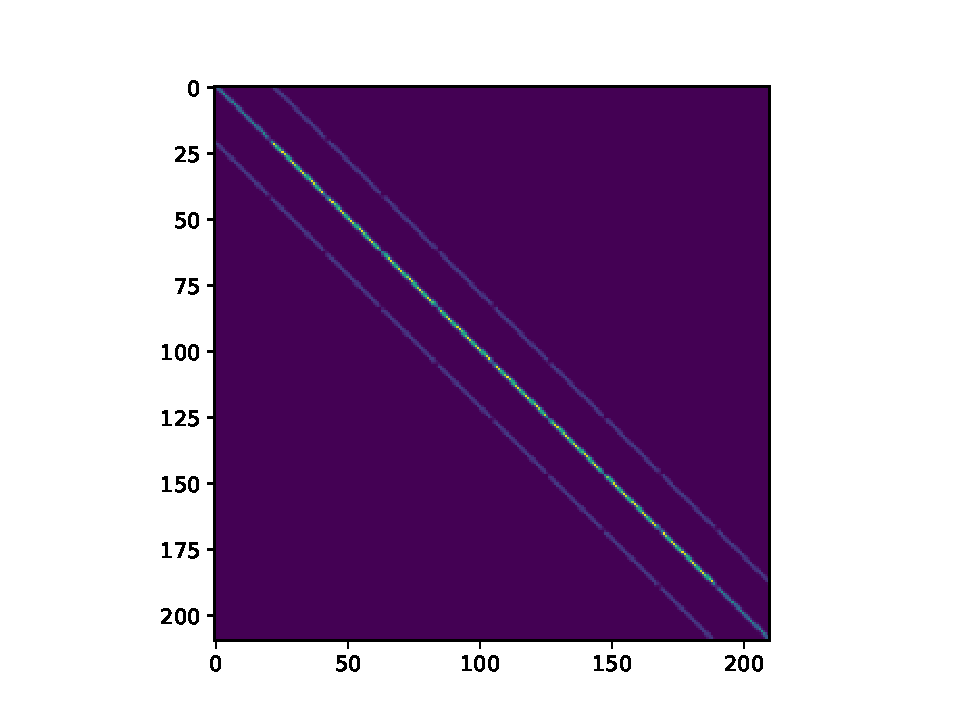
\includegraphics{heat_files/figure-latex/unnamed-chunk-1-3.pdf}

\begin{minted}[autogobble]{python}
to_fix = np.where(points[:, 0] == 0)[0]
S[to_fix, :] = np.eye(dofs)[to_fix, :]
RHS[to_fix] = 1

to_fix = np.where(points[:, 0] == Lx)[0]
S[to_fix, :] = np.eye(dofs)[to_fix, :]
RHS[to_fix] = 0

x = np.linalg.solve(S, RHS)

plt.tripcolor(points[:,0],points[:,1],elements,x,shading='gouraud')
plt.show()
\end{minted}

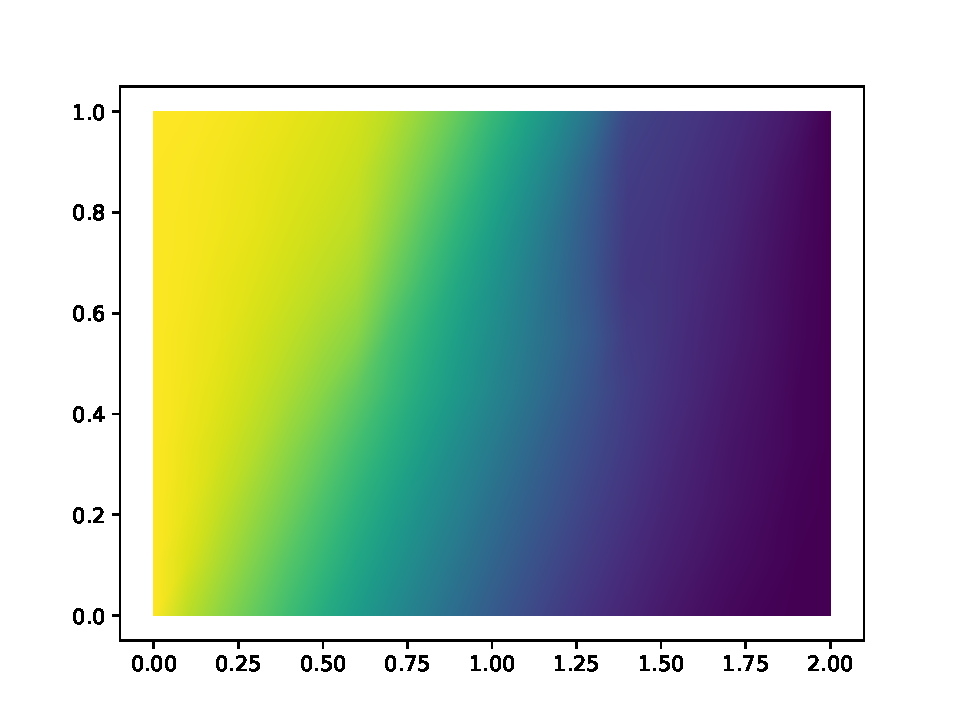
\includegraphics{heat_files/figure-latex/unnamed-chunk-1-4.pdf}
